\documentclass[9pt]{beamer}
\usepackage[utf8]{inputenc}
\usepackage{gensymb}
\usepackage{amsmath}
\usepackage{amssymb}
\usepackage{float}
\usepackage{graphicx}
\usepackage{hyperref}
\usepackage{appendix} 
\usepackage[export]{adjustbox}
\usepackage{makecell}
\usepackage{graphicx}
\usepackage{multimedia}
\usepackage[font=scriptsize]{caption}
\usetheme{Boadilla}

%\setbeamersize{text margin left=0mm,text margin right=30mm} 

\begin{document}

\title{Project Presentation}
\author[]{Gabriel Beauplet}
\date{Friday November 2} 
%\titlegraphic{\includegraphics[scale=0.3]{../Images/logo_prez}}
\maketitle

\begin{frame}
\frametitle{Introduction}
\begin{block}{The ScanAllFish project}
\begin{itemize}
\item Creating a freely available database of scans of all the world’s 30,000 fish species
\begin{itemize}
\item Problem 1 : Micro-CT devices are expensive
\item Problem 2 : One scan may last up to 12h
\end{itemize}
\item Solution : Scan several fishes simultaneously
\end{itemize}
\end{block}
\begin{block}{TopoAngler}
\begin{itemize}
\item Utilizing topological analysis to create selectable candidate features
\item Providing an intuitive user-interface
\item The ability to export all selected meta-features for further analysis
\end{itemize}
\end{block}
\end{frame}

\begin{frame}
\frametitle{Topological Analysis}
\framesubtitle{Join tree}
\begin{block}{Level set topology}
The super level set of a real value $a$ is $\{x\in \mathbb{R}^3 | f(x)\geq a\}$
\end{block}
\begin{block}{Join tree}
We sweep the 3D space by decreasing the function value f\\
For each vertex encountered, the topological change caraterize the vertex, it can be :
\begin{itemize}
\item regular : The topology of the super-level sets do not change.
\item maximum: A new super-level set component is created.
\item join saddle: Two super-level set components merging.
\end{itemize}
A vertex that is not regular is called critical.
\end{block}
\begin{figure}
\centering
\begin{minipage}{.5\textwidth}
  \centering
  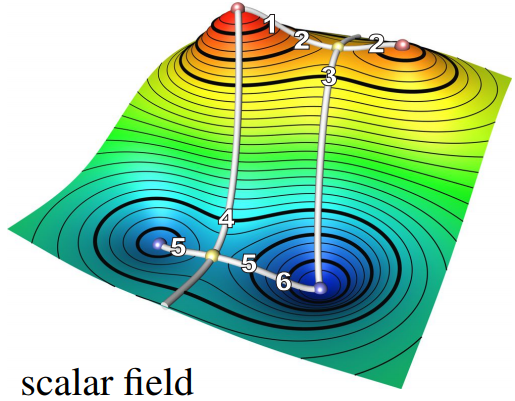
\includegraphics[width=0.4\linewidth]{Images/scalar_field}
%  \captionof{figure}{3D grid}
\end{minipage}%
\begin{minipage}{.5\textwidth}
  \centering
  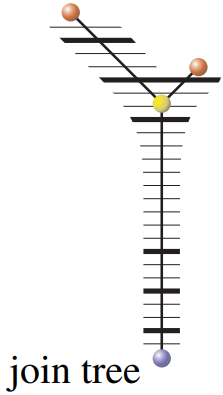
\includegraphics[scale=0.15]{Images/join_tree_of_scalar_field}
%  \captionof{figure}{/Tetrahedron}
\end{minipage}
\end{figure}
\end{frame}

\begin{frame}
\frametitle{Topology-based Segmentation}
%\begin{block}{Definition}
%For a vertex v, the \textbf{upper link} is defined as the sub-graph induced by adjacent vertices having a function value greater than v
%\end{block}
\begin{block}{Upper link}
For a vertex v, $\{u \in N(v) |f(u)\geq f(v\})$
\end{block}
\begin{block}{Computing the augmented join tree}
The algorithm first sorts the vertices of K by decreasing function value
\begin{enumerate}
\item If the upper link of v is empty, then create a new component containing v and set v as its head
\item If the upper link of v is not empty, find the components that contain the vertices in the upper link of v. Add an edge between v and the head of each of the components. Next, merge these components and set v as the head of the merged component.
\end{enumerate}
\end{block}
%\begin{block}{Computing the join tree}
%\begin{itemize}
%\item The regular vertices form degree-2 nodes in the augmented join tree.
%\item The join tree is then computed by merging (removing) the regular nodes
%from the augmented join tree  
%\end{itemize}
%\end{block}
\begin{figure}
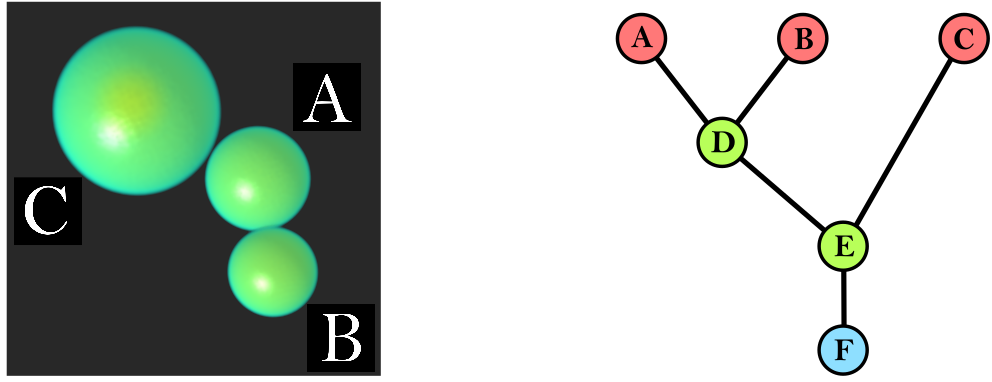
\includegraphics[scale=0.15]{Images/join_tree}
\caption{Left : A level set at a given real value is corresponds to the shown spherical surfaces. A super-level set corresponds to the region inside the three spheres. Right : The join tree of the scalar function}
\end{figure}
\end{frame}

\begin{frame}
\frametitle{Hierarchical Segmentation}
\begin{block}{Principle}
\begin{itemize}
\item Two types of importance measure
\begin{itemize}
\item $|f(c_1)-f(c_2)|$ where ($c_1$,$c_2$) is an edge
\item Edge Hypervolume (the integral of the scalar function over the enclosed volume)
\end{itemize}
\item All leaf edges that are incident on a maximum, are first added to a priority queue based on the importance measure
\item Then, at each step, the least important leaf edge is removed
\end{itemize}
\end{block}
\begin{figure}
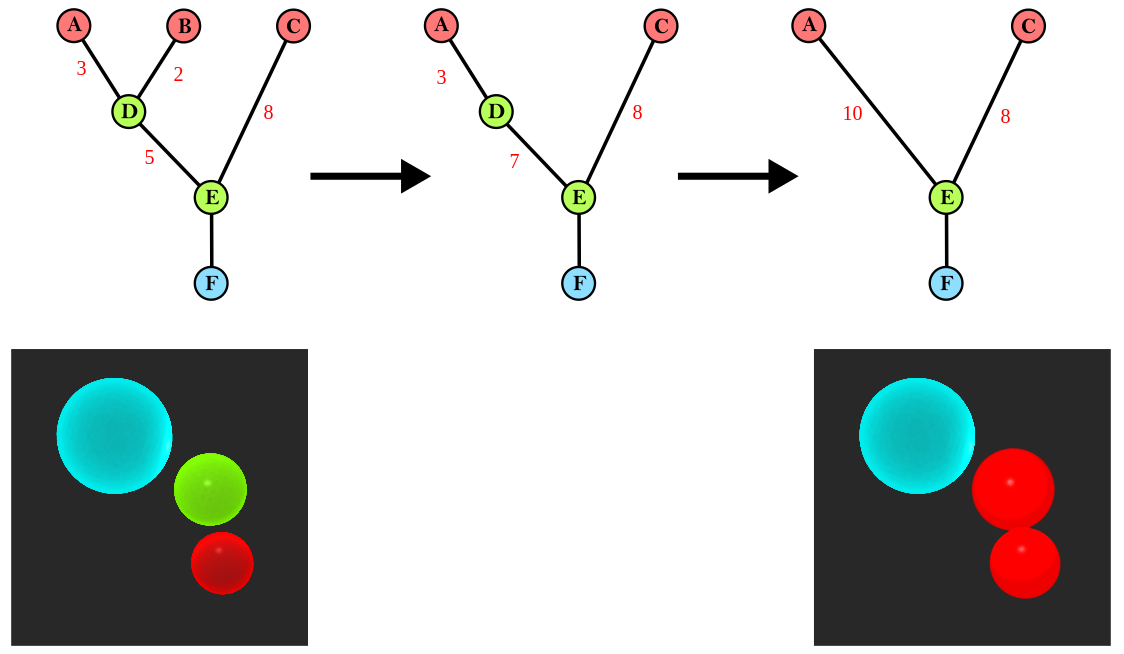
\includegraphics[scale=0.15]{Images/join_tree2}
\caption{A hierarchical segmentation of the volume is performed using the join tree. By increasing the simplification level (top), different branches of the tree are joined to form a simplified represtation. This corresponsd to the number of features that are shown in the rendering (bottom).}
\end{figure}
\end{frame}

\begin{frame}
\frametitle{Hierarchical Segmentation}
\begin{block}{Computing hierarchical segmentation}
\begin{itemize}
\item The user select a number n of candidate features
\item Only the n most important features are kept, the other are removed
\end{itemize}
\end{block}
\begin{figure}
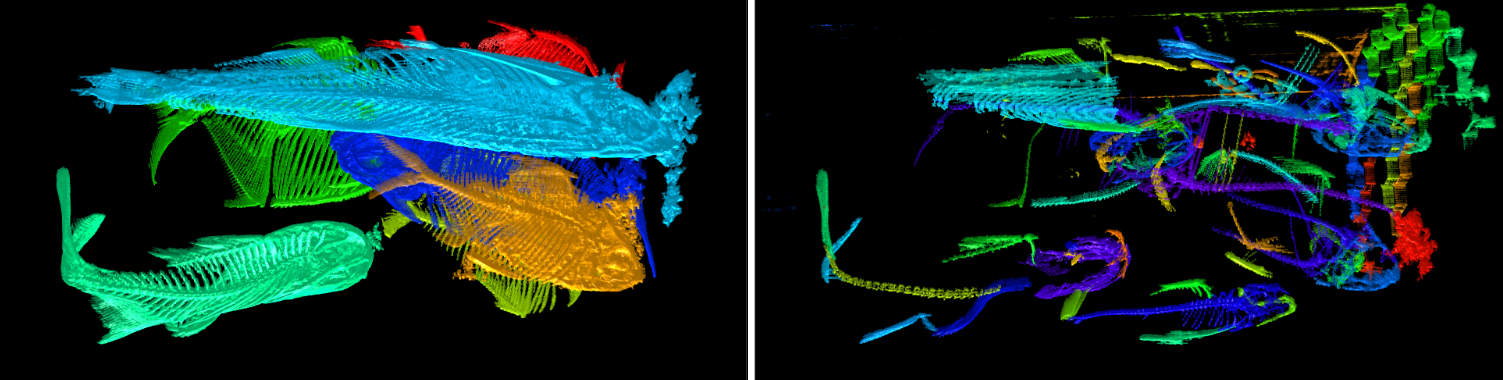
\includegraphics[scale=0.2]{Images/features_simplification}
\caption{Selecting a different number of candidate features leads to a change in granularity of detected features. Changing between different simplifications is required by the workflow in order to construct entire fishes with the necessary detail.}
\end{figure}
\end{frame}

\begin{frame}
\frametitle{My implementation}
\begin{block}{Make the dataset}
\begin{itemize}
\item Collect the data : Took 3 fishes on the ScanAllFish project webpage
\begin{itemize}
\item Each fish is contains around 1 billion points
\end{itemize}
\item Downsample each dimension by 8
\item Stack the 3 fishes
\end{itemize}
\end{block}

\begin{block}{The algorithm}
\begin{itemize}
\item Implementation of the H.S. using Python and Cython
\begin{itemize}
\item Compute the join tree
\item Delete all the maximum until n are left
\end{itemize}
\end{itemize}
\end{block}

\begin{block}{After the algorithm}
\begin{itemize}
\item Upsample each volume segmented
\item Extract the minimum volume containing each volume segmented
\end{itemize}
\end{block}

\end{frame}

\begin{frame}
\frametitle{Results}
\begin{figure}
\centering
\begin{minipage}{.5\textwidth}
  \centering
  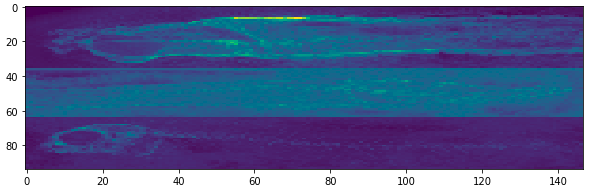
\includegraphics[scale=0.3]{Images/fish_superposition}
  \captionof{figure}{Superposition of 3 fishes}
\end{minipage}%
\begin{minipage}{.5\textwidth}
  \centering
  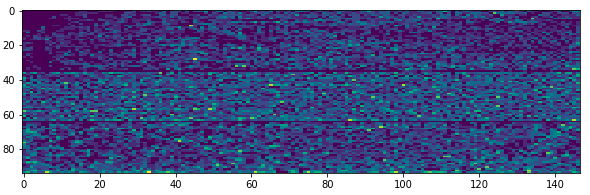
\includegraphics[scale=0.3]{Images/9648_fishes_separation}
  \captionof{figure}{Separation in 9648 parts}
\end{minipage}
\end{figure}

\begin{figure}
\centering
\begin{minipage}{.5\textwidth}
  \centering
  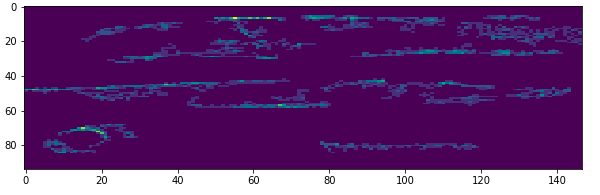
\includegraphics[scale=0.3]{Images/35_fishes_separation}
  \captionof{figure}{Separation in 35 parts}
\end{minipage}%
\begin{minipage}{.5\textwidth}
  \centering
  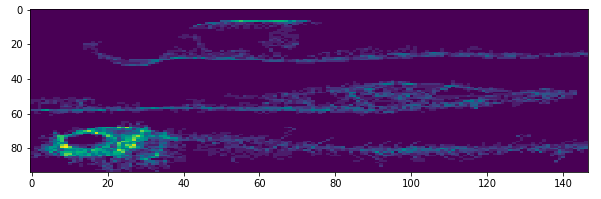
\includegraphics[scale=0.3]{Images/3_fishes_separation}
  \captionof{figure}{Separation in 3 parts}
\end{minipage}
\end{figure}
\begin{figure}
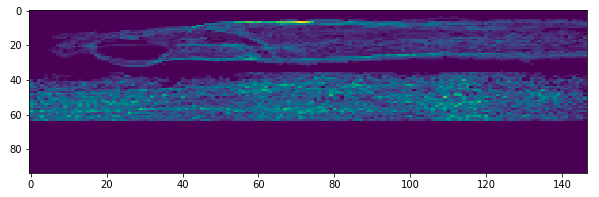
\includegraphics[scale=0.3]{Images/2_fishes_separation}
\caption{Separation in 2 parts}
\end{figure}
\end{frame}

\begin{frame}
\frametitle{Comparison of the importance measure}
\begin{block}{}
\begin{itemize}
\item Using the sum as importance measure gives better segmentation
\end{itemize}
\end{block}
\begin{figure}
\centering
\begin{minipage}{.5\textwidth}
  \centering
  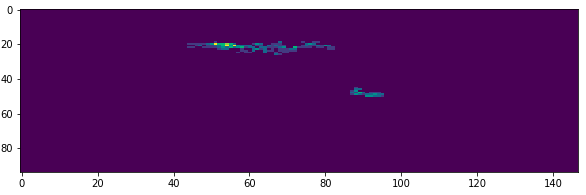
\includegraphics[scale=0.25]{Images/max_3_separation}
  \captionof{figure}{Separation in 3 parts using the absolute difference between the maximum values of a maximum component and the maximum value of his parent}
\end{minipage}%
\begin{minipage}{.5\textwidth}
  \centering
  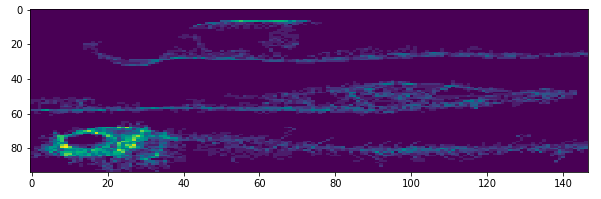
\includegraphics[scale=0.27]{Images/3_fishes_separation}
  \captionof{figure}{Separation in 3 parts using the sum of each maximum component}
\end{minipage}
\end{figure}
\end{frame}

\begin{frame}
\frametitle{Encountered problems}
\begin{block}{Quotes from the TopoAngler paper}
\begin{itemize}
\item \textit{If the upper link of v is not empty, find the components that
contain the vertices in the upper link of v}
\item \textit{A consistent comparison between vertices is ensured by a simulated perturbation of the function}
\end{itemize}
\end{block}
\end{frame}


\begin{frame}
\frametitle{Marching Cubes}
\begin{figure}
\centering
\begin{minipage}{.5\textwidth}
  \centering
  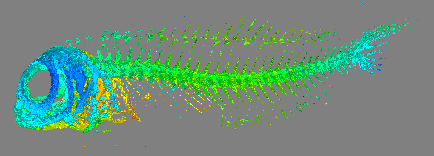
\includegraphics[scale=0.3]{Images/mayavi}
  \captionof{figure}{Mesh of the extracted fish using the marching cube algorithm}
\end{minipage}%
\begin{minipage}{.5\textwidth}
  \centering
  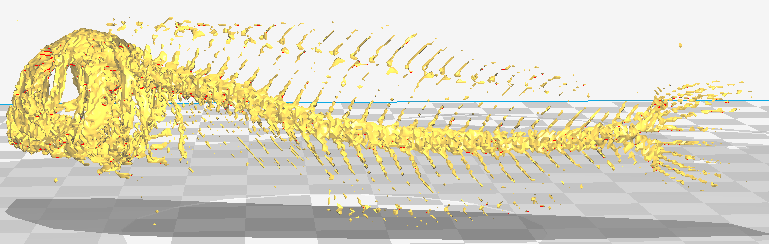
\includegraphics[scale=0.22]{Images/cura_fish}
  \captionof{figure}{Mesh of the fish before adding support}
\end{minipage}
\end{figure}
\begin{figure}
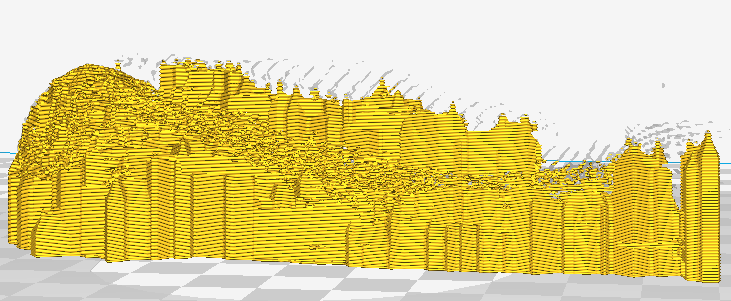
\includegraphics[scale=0.2]{Images/cura_supports}
\caption{Mesh of the fish after adding support}
\end{figure}
\end{frame}

\begin{frame}
\frametitle{Animation}
\framesubtitle{Moving the fin}
\begin{figure}
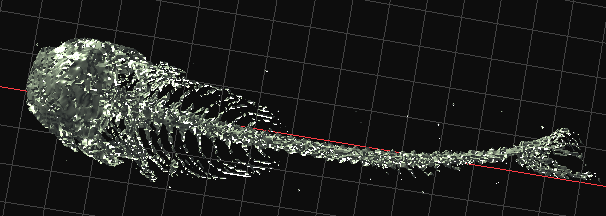
\includegraphics[scale=0.3]{Images/fish_from_top}
\caption{Image of the fish from top after the extraction}
\end{figure}
\begin{figure}
\centering
\begin{minipage}{.5\textwidth}
  \centering
  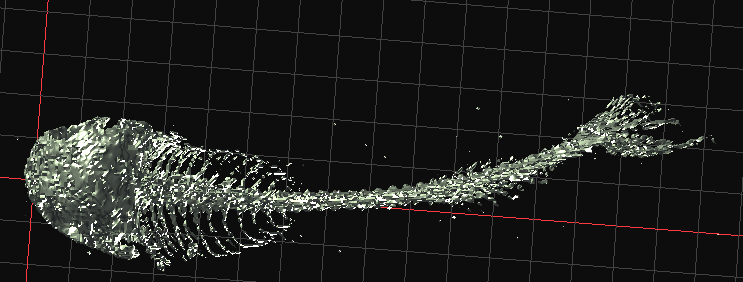
\includegraphics[scale=0.2]{Images/left_fin}
  \captionof{figure}{Start position of the fin using the formula for each point p : $x(p)=5.10^{-4}z(p)^2$}
\end{minipage}%
\begin{minipage}{.5\textwidth}
  \centering
  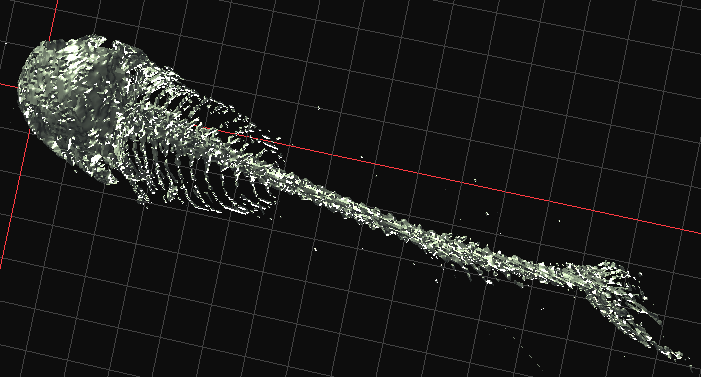
\includegraphics[scale=0.22]{Images/right_fin}
  \captionof{figure}{End position of the fin using the formula for each point p : $x(p)=-7.10^{-4}z(p)^2$}
\end{minipage}
\end{figure}
\end{frame}

\begin{frame}
\frametitle{Animation}
\framesubtitle{Bad moving of the fin}
\begin{figure}[h!]
\centering 
\movie[label=show3,poster,autostart,showcontrols,loop] 
  {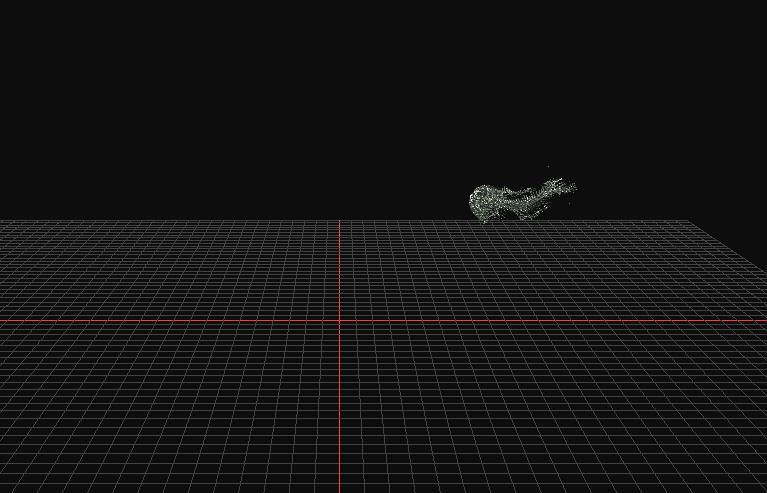
\includegraphics[width=0.8\textwidth]{Images/random_swim}}{Images/swim_mirror.mp4}
  \caption{Example of random swim}
 \end{figure} 
\end{frame}

\begin{frame}
\frametitle{Animation}
\framesubtitle{Fish Game}
%\begin{block}{What we have}
%\begin{itemize}
%\item Move the fin
%\item Move on the whole fish (by translation)
%\item Orient the whole fish (by rotation)
%\end{itemize}
%\end{block}
\begin{block}{What could we do ?}
\begin{itemize}
\item Move the fish randomly in the 3D space
\item A game : The fish Game (analogy with the snake game)
\begin{itemize}
\item Move the fish with the left and right arrow keys
\item Eat the food to get a bigger fish
\item The game stops if you touch the edges with the head of the fish
\end{itemize}
\end{itemize}
\end{block}
\begin{figure}[h!]
\centering 
\movie[label=show3,poster,autostart,showcontrols,loop] 
  {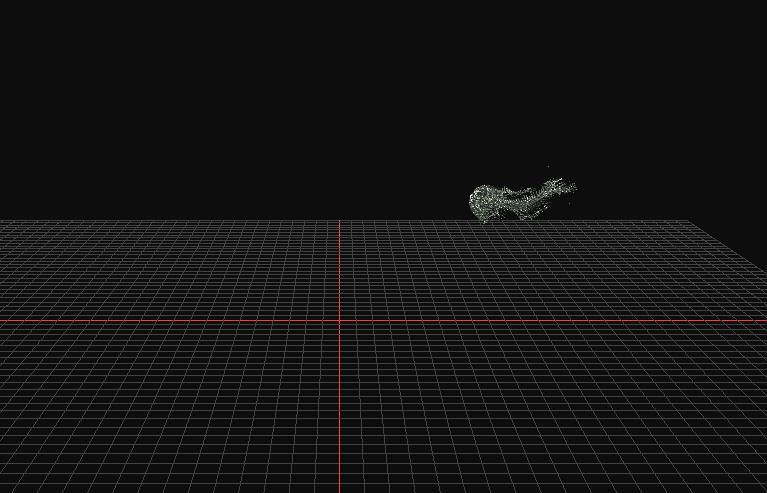
\includegraphics[width=0.6\textwidth]{Images/random_swim}}{Images/fish_moving.mp4}
  \caption{Example of random swim}
 \end{figure} 

\end{frame}

\begin{frame}
\frametitle{Conclusion}
\begin{block}{Improvement}
\begin{itemize}
\item Try to improve the hierarchical segmentation with machine learning
\item Make the fish game with 3 degrees of liberty
\item Make the fish open his mouth
\item Add other fishes
\end{itemize}
\end{block}
\begin{figure}
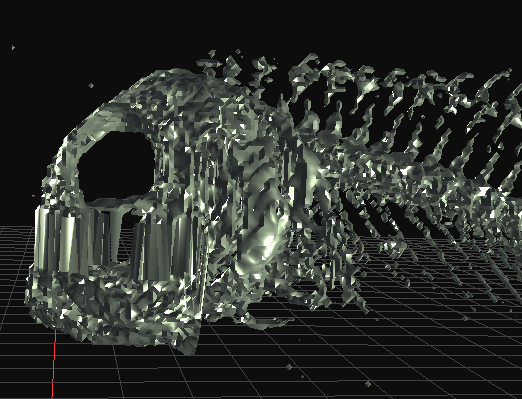
\includegraphics[scale=0.2]{Images/open_mouth}
\caption{Result when you lower one part of the fish head}
\end{figure}
\textbf{All the code is available on my github page : https://github.com/beaupletga
}\end{frame}

\end{document}
